\chapter{Konzeption}
\label{chap:Konzeption}

Dieses Kapitel beschreibt die Resultate und Ergebnisse aus der Konzeptionsphase. Nachfolgend werden auf die verschiedenen Konzeptionsvarianten eingegangen. Dabei werden Überlegungen und Bezüge zur Aufgabenstellung gemacht. Jede Variante wird abschliessend mit einem kurzen Fazit beurteilt

\section{Konzeptionsgrundlage}
\label{sec:Konzeptiongrund}
Als Konzeptionsgrundlage dient das Pflichtenheft, welches im Anhang \todo{referenz} einsehbar ist. Wie darin erwähnt, soll das Modul möglichst frei drehend konzipiert werden. Dies ist das ausschlaggebendste Kriterium für die Bauform des Moduls. Da der Velodyne VLP-16, wie in Kapitel \ref{subsec:Velodyne} erläutert, einen begrenzten vertikalen Öffnungswinkel besitzt, wurde bei den folgenden Konzepten die Möglichkeit eines beweglichen Moduls geprüft. Durch eine grösseren Öffnungswinkel kann während der Bewegung der Raum besser ausgeleuchtet werden. Ein weiteres relevantes Kriterium ist die Einsatzmöglichkeit des Modul. Es soll einerseits auf dem Packbot, sowie auch als eigenständiges Produkt funktionieren. Daher sind als Schnittstellen einen Speiseanschluss, welcher 12 Volt DC liefert und eine Ethernet RJ45-Anschluss nötig. Nachfolgend sind auf diesen Grundlagen drei Varianten dargelegt.

\section {Variante 1: Plattform}
\label{sec:var1}
Die Variante 1: Plattform ist in der Skizze in Abbildung \ref{fig:plattform} ersichtlich. Bei dieser Konstruktion werden alle elektronischen Komponenten, welche für die Signalverarbeitung und die Energieversorgung nötig sind, in einem rechteckigen Gehäuse im unteren Teil verbaut. Die Interface Box des Velodyne VLP-16 wird auch in diesem Gehäuse untergebracht. Lediglich der Laserscanner VLP-16 befindet sich ausserhalb des Gehäuses auf der Plattform oberhalb des Gehäuses.

\begin{figure}[H]
	\centering
	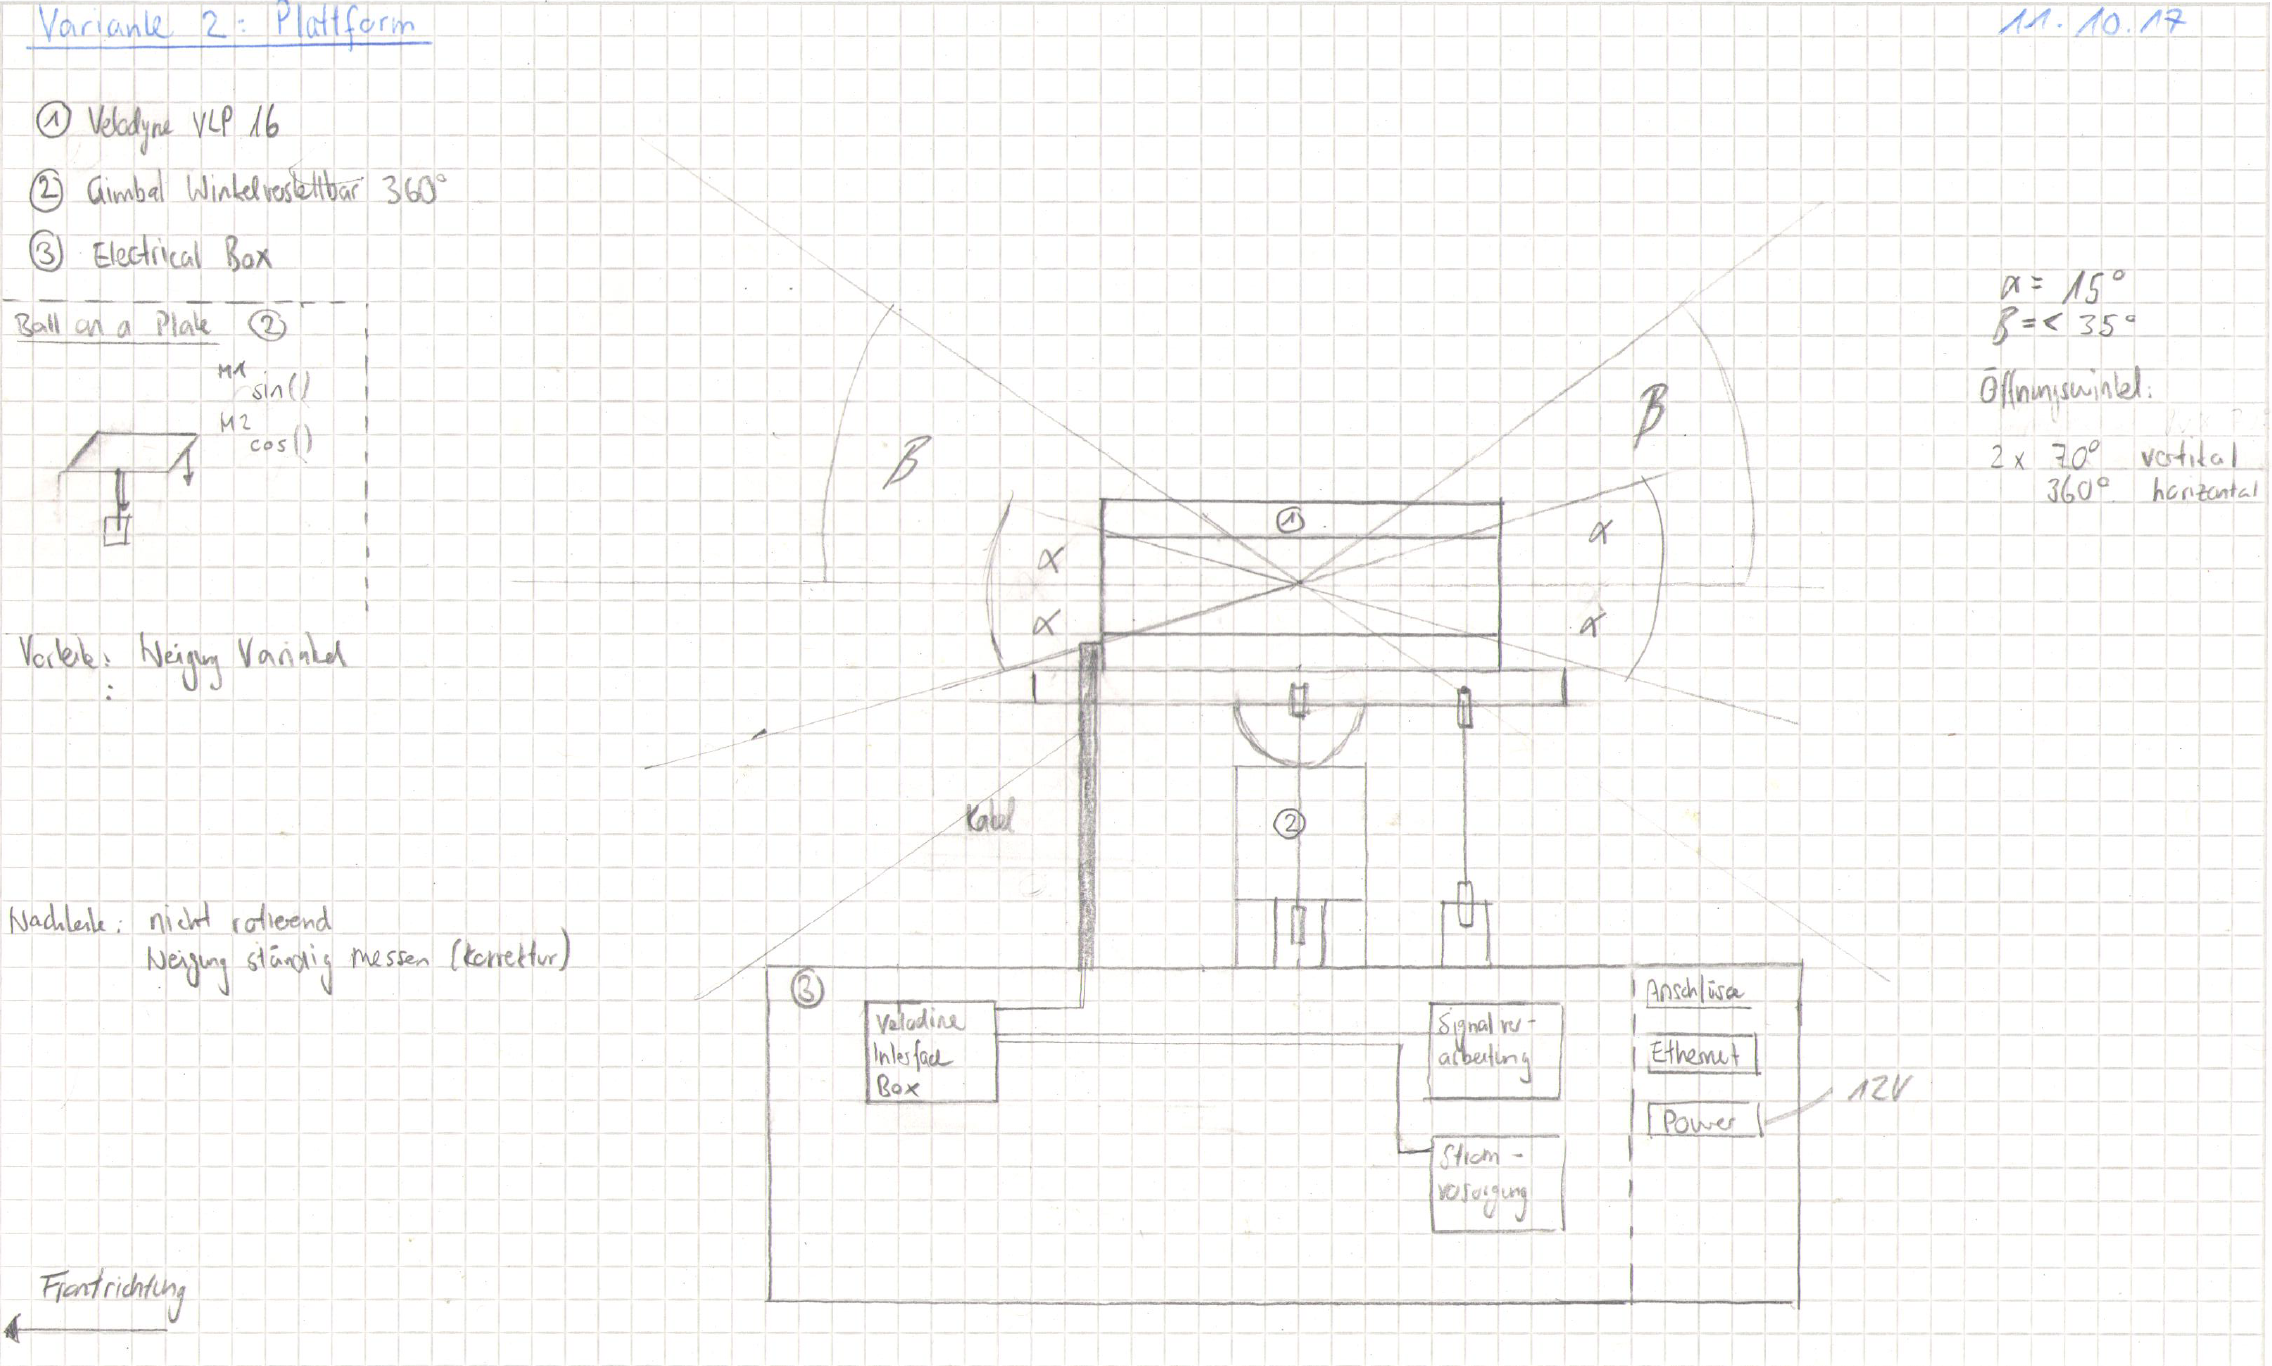
\includegraphics[width=1\textwidth]{resources/skizzev1.PNG}
	\caption{Skizze Variante 1}
\label{fig:plattform}
\end{figure} 
	
 Die Eigenheit dieser Konzeption ist die Plattform, auf welcher sich der Velodyne VLP-16 befindet. Der Einsatz dieser Plattform erklärt sich durch ein bekanntes Regelungsexperiment namens "Ball on a Plate". In Abbildung \ref{fig:BalllonaPlateCAD}ist eine CAD-Zeichnung eines solchen Regelungsexperiment dargestellt. Bei "Ball on a Plate" werden zwei Servomotoren, welche je mit einem Gelenk mit ieiner Seite der Plattform verbunden sind, angesteuert. Indem die Servomotoren mittig auf der Seite mit der rechteckigen Plattform verbunden sind, kann durch Drehen der Servomotoren die Plattform zweiachsig geneigt werden. Im Regelungsexperiment kann durch Zuhilfenahme einer PID-Regelung ein Ball darauf balanciert werden. 
 
\begin{figure}[H]
	\centering
 	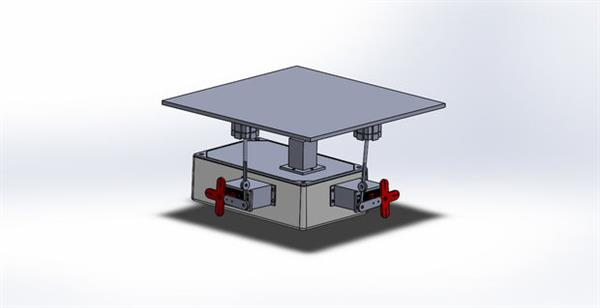
\includegraphics[width=1\textwidth]{resources/ballonaplate_cad}
	\caption{Ball on a Plate CAD {\cite{ballonaplate}}}
	\label{fig:BalllonaPlateCAD}
\end{figure} 

 Diese Überlegungen bieten die Möglichkeit den Laserscanner VLP-16, welcher in der Konzeption auf der Plattform befestigt ist, durch das Ansteuern der Servomotoren in alle Richtungen zu neigen. Somit kann  der Öffnungswinkel in jede Richtung vergrößert werden. Die Grenzen liegen dabei im wesentlichen bei der mechanischen Begrenzung.
 
 Hauptproblematik bei dieser Konzeption ist die zusätzlich nötige Sensorik. Durch die Neigung der Plattform kann ohne zusätzliche Sensorik nicht auf die Transformationsebenen zurück geschlossen werden. Dies erschwert die Visualisierung der 3D-Laserscanner Messdaten. Die Plattform müsste mittels einer eigenen \ac {IMU}, welche aus Gyrosensor, Accelerometer und Magnetometer besteht, erweitert werden. Zusätzlich ist die Realisierung der Konzeption sehr stark abhängig von den mechanischen Komponenten, da die Verbindungsstifte von Servomotor und Grundplatte die Winkeländerung festlegen.
 
 Während der Besprechung mit Herr Jensen vom \todo{ZEIT} wurde diese Konzeption verworfen und nicht mehr weiter vertieft.
 

\section {Variante 2: Turm stationär}
\label{sec:var2}

\begin{figure}[H]
	\centering
	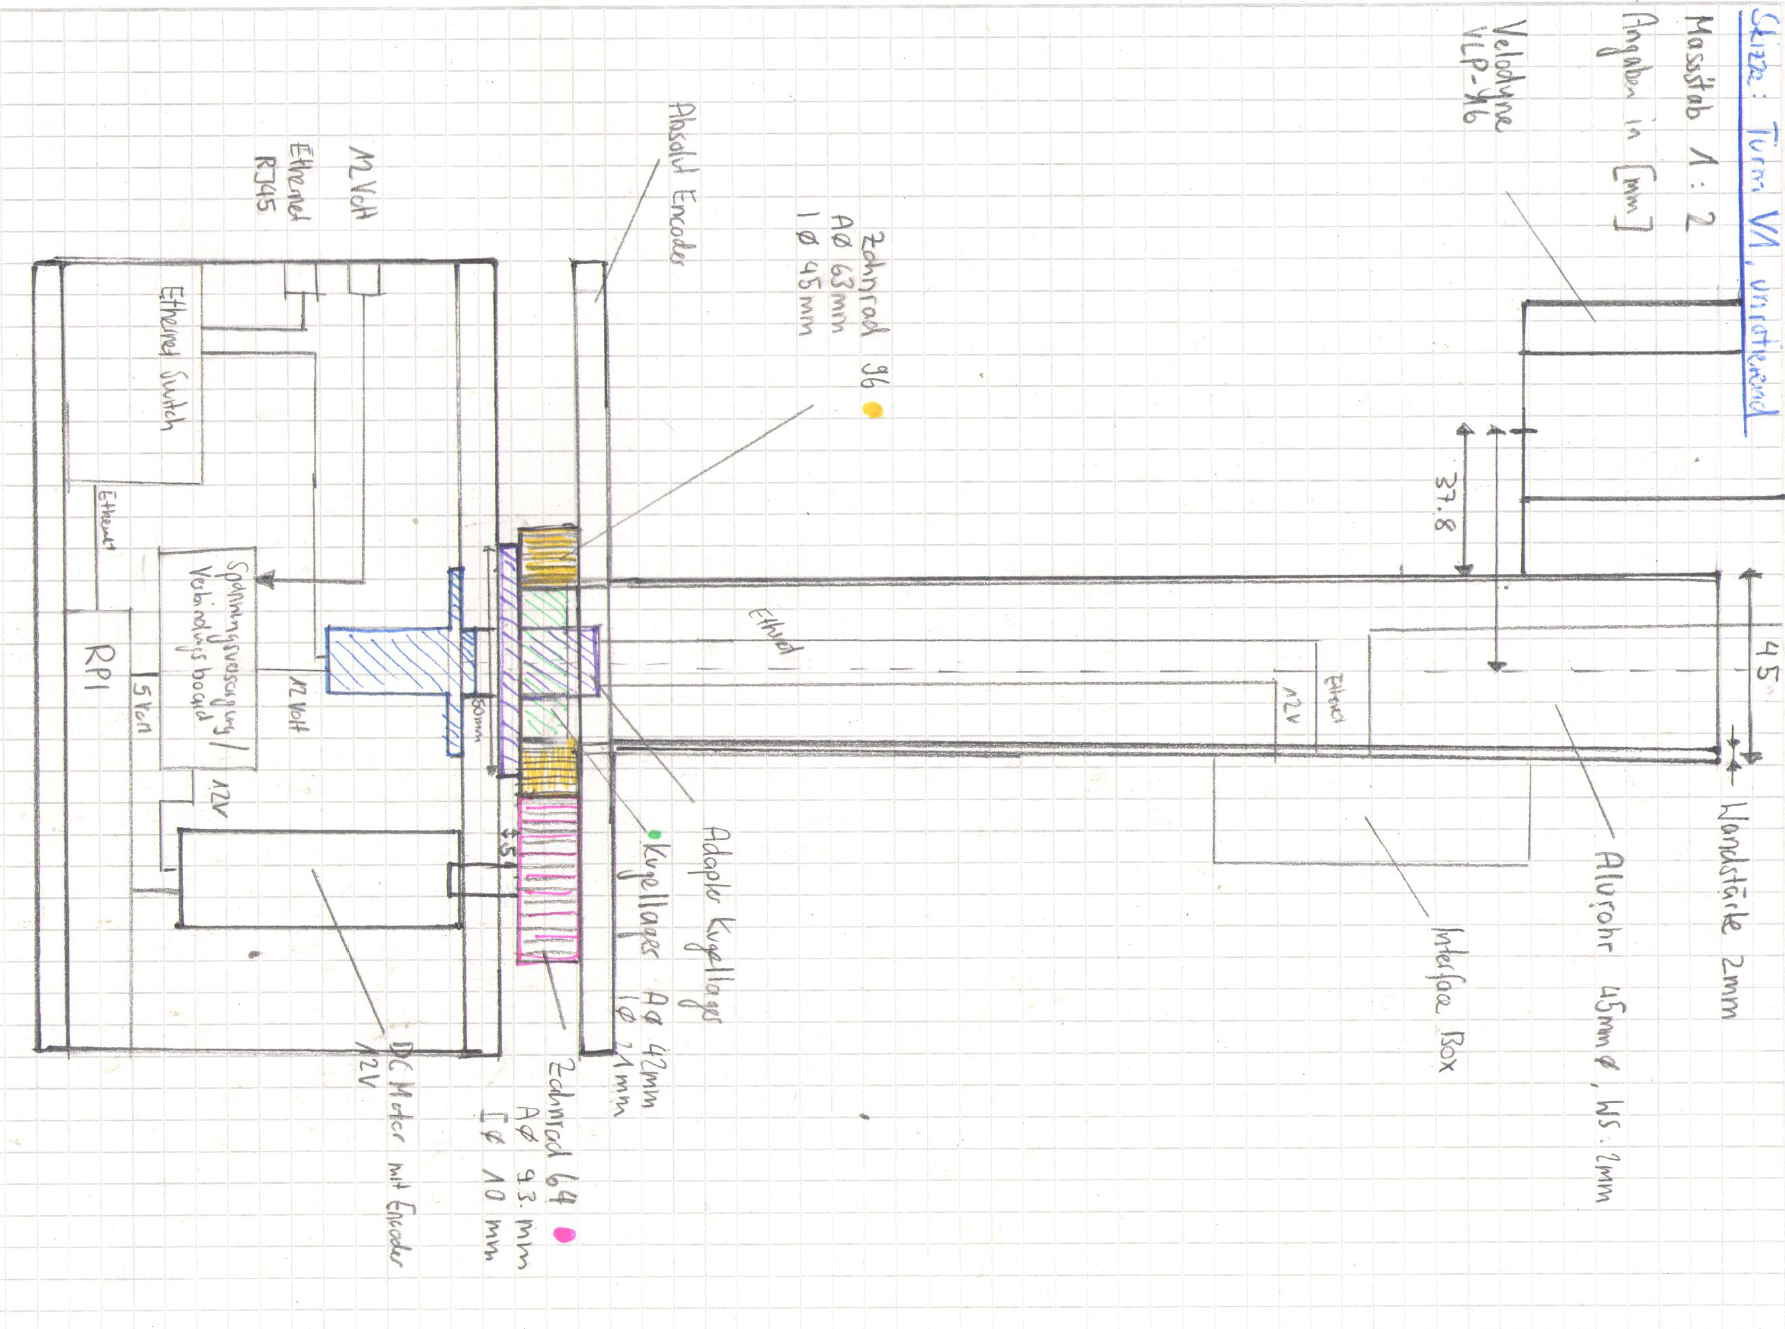
\includegraphics[angle=90,width=0.8\textwidth]{resources/skizze_unrotierend.PNG}
	\caption{Skizze Variante 2 }
	\label{fig:skizze_unrotierend}
\end{figure} 

Das zweite Konzept ist eine Turmartige Konstruktion, die in Abbildung \ref{fig:skizze_unrotierend} dargestellt ist. Die Idee dazu lieferte das TEAM IMM an der \ac{ENRICH} 2017. Dabei befindet sich der Velodyne VLP-16 abgesetzt von den elektrischen Komponenten in der Höhe. Dies ermöglicht einen größeren Erfassungswinkel. Speziell an diesem Konzept ist, dass sich der Turm endlos drehen lässt. Diese Konfiguration verbessert die Problematik des Velodyne, welche in \ref{subsec:Velodyne} erläutert ist. Durch die interne Rotation des VLP-16 kann ein Raum in dieser Konfiguraton die Vertikale grösstmöglich auflösen. Die Horizontale Abdeckung liegt nur bei 2 * 30 Grad, doch durch die zusätzliche Rotierung des Moduls kann durch eine 180 Grad Drehung eine komplette Raumwahrnehmung entstehen.

In dieser Konfiguration wird der VLP-16 mit einem Gleichstrommotor, der über zwei Zahnräder mit dem Alurohr verbunden ist, gedreht. Der untere Teil des Moduls, in dem sich die Datenverarbeitung befindet, ist stationär. Mittels einem Adapter, an dem ein Kugellager befestigt ist, kann ein möglichst geringe Reibung erzielt werden.

Die gesamte Datenverarbeitung und Ansteuerung wird im stationären Teil getätigt. Die Kabelverbindung des VLP-16 wird über einen Schleifring nach unten geführt. 

Nachteil dieser Konfiguration ist, dass es schlecht erweiterbar ist. Da der Schleifring begrenzte Kabeldurchführungen besitzt können keine weiteren Komponenten wie beispielsweise die 3D Kamera Theta hinzugefügt werden. Ein weiterer Nachteil ist die Problematik, wenn die Rotationsgeschwindigkeit des Turm auf mehrere Umdrehungen pro Sekunde ansteigt. Es können fehlerhafte Messresultate beim VLP-16 entstehen, daher muss die Drehgeschwindigkeit des Turms verhältnismässig langsam gegenüber der Drehgeschwindigkeit VLP-16 sein.


\section {Variante 3: Turm rotierend}
\label{sec:var3}
Das dritte Konzept ist wiederum eine Turmartige Konstruktion.Eine Skizze ist in Abbildung \ref{fig:skizze_rotierend} ersichtlich. Es handelt sich hier um eine abgeänderte Version von Variante 2. Dabei befindet sich der Velodyne VLP-16 erneut abgesetzt von den elektrischen Komponenten in der Höhe. Die wesentlichste Änderung liegt darin, dass nun auch die Datenverarbeitung im unteren Teil mitdreht. Dies wurde ermöglicht indem alle mechanischen Drehkomponenten und der DC Motor umgedreht wurden. Somit kann das Problem der Erweiterbarkeit des vorherigen Konzepts gelöst werden. Die gesamte Elektronik und Sensorik dreht nun mit. Lediglich die Schnittstellen Ethernet und 12 Volt Speisung führen über den Schleifring zum Packpot. 
Für diese Konfiguration wird lediglich ein Alusockel benötigt, welche das Alurohr mit dem Gehäuse verbindet.


\begin{figure}[H]
	\centering
	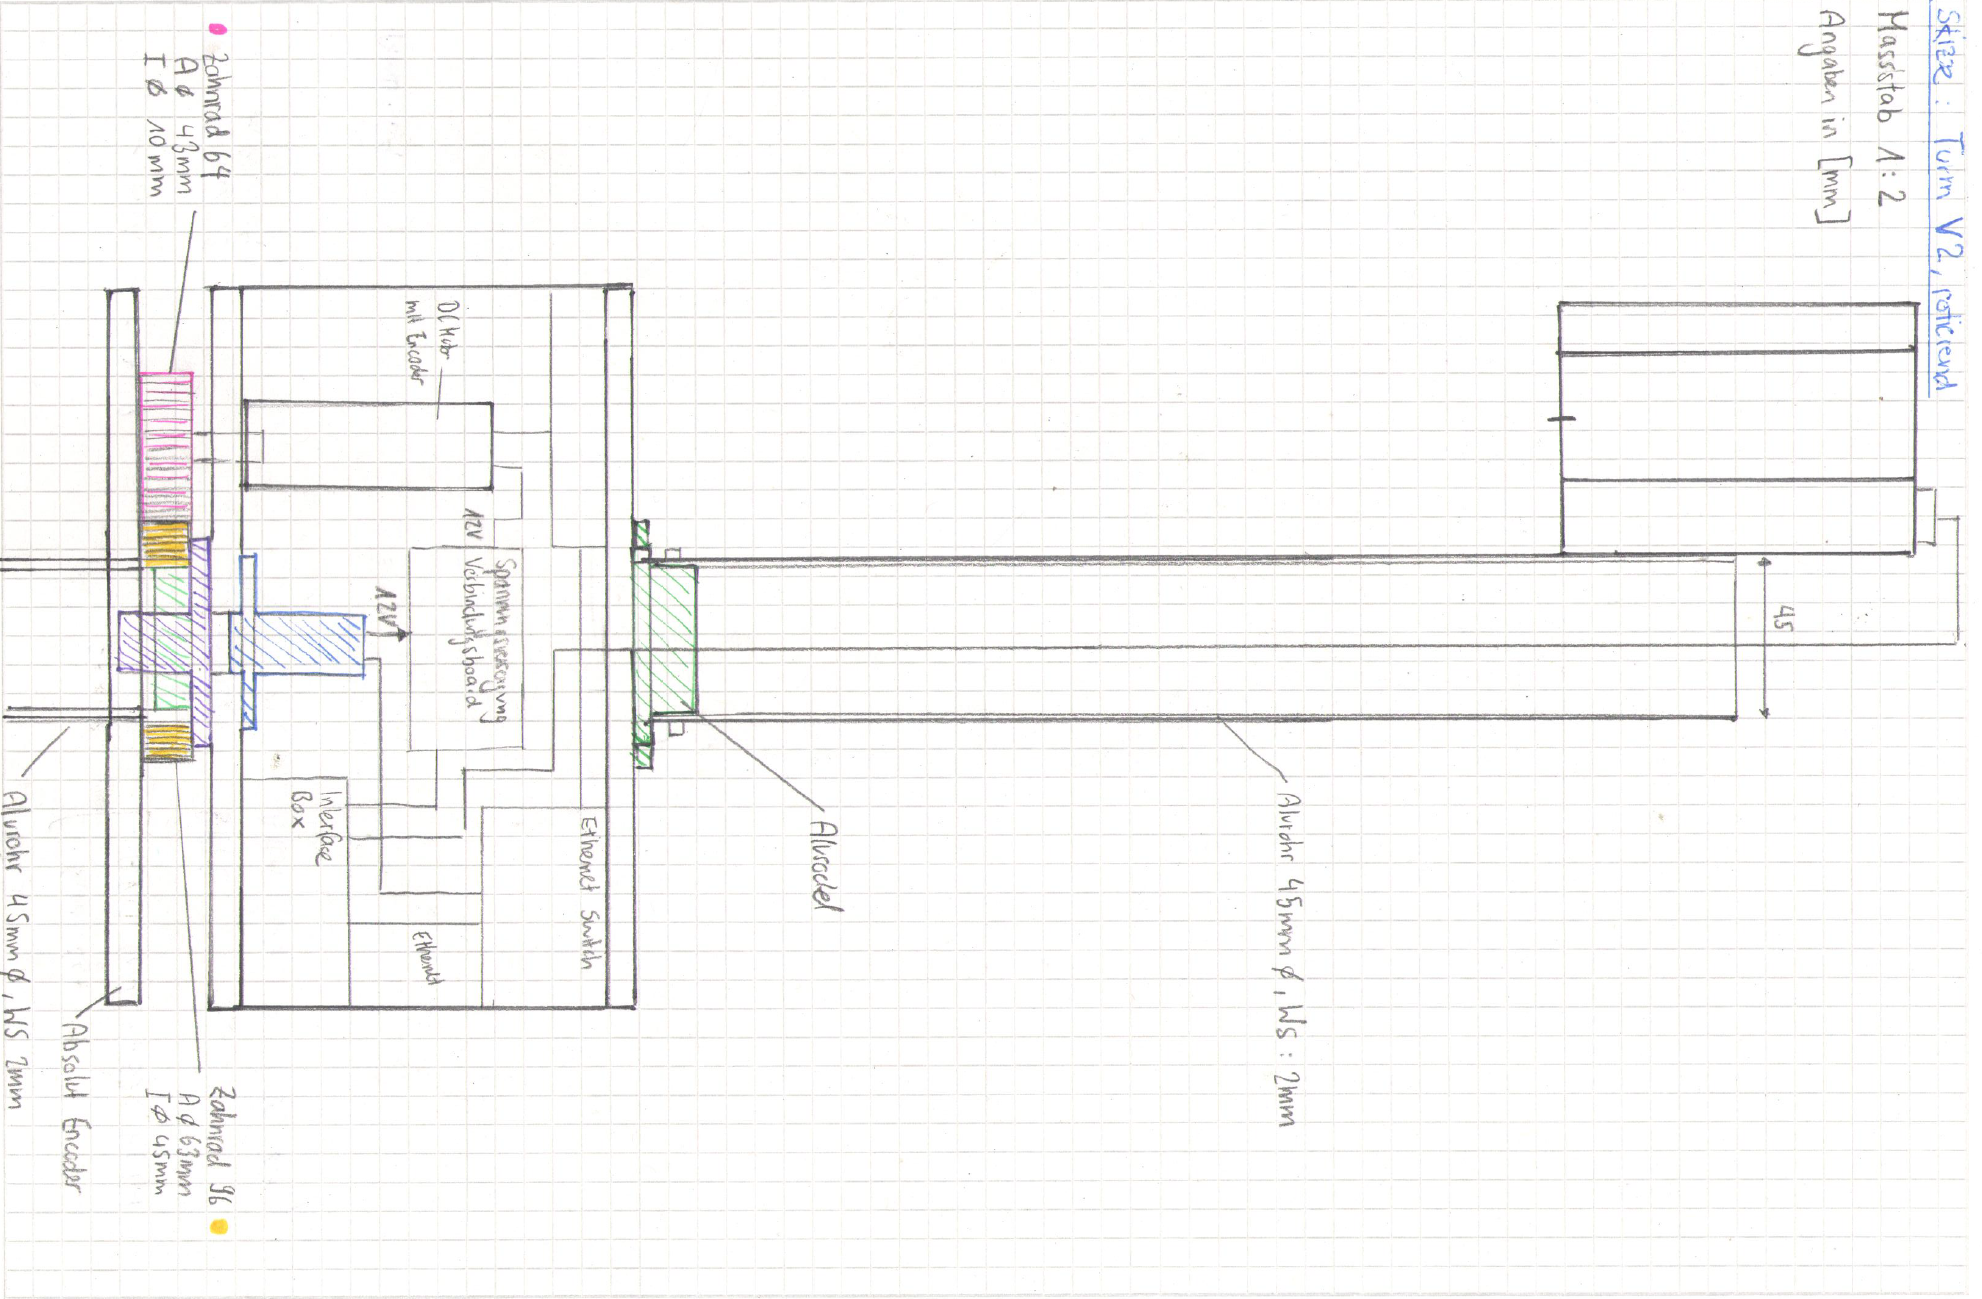
\includegraphics[angle=90,width=0.7\textwidth]{resources/skizze_rotierend.PNG}
	\caption{Skizze Variante 3 }
	\label{fig:skizze_rotierend}
\end{figure} 

\section {ausgewählte Komponenten}
\label{sec:ausgewählteKomponenten}

\section{Zwischenfazit}
\label{ZwischenfazitKonz}

